include(`macros.m4')

\pdfbookmark[1]{standard file descriptors}{stdfds}

\begin{slide}
\sltitle{File API}
\begin{itemize}
\item before working with a file, it must be first opened via
\funnm{open}() or \funnm{creat}()
\item open files are accessible via \emph{file descriptors}, numbered from 0.
More descriptors can share the same file opening (read/write mode, position).
\item standard file descriptors
    \begin{itemize}
    \item 0 \dots{} standard input (read only)
    \item 1 \dots{} standard output (write only)
    \item 2 \dots{} unbuffered error output (write only)
    \end{itemize}
\item for reading and writing a file: \funnm{read}(), \funnm{write}()
\item position change: \funnm{lseek}(), close: \funnm{close}(),
information: \funnm{stat}(), file control: \funnm{fcntl}(),
access rights: \funnm{chmod}(), \dots
\end{itemize}
\end{slide}

\begin{itemize}
\item Every function that allocates file descriptors (not just \funnm{open}() or
\funnm{creat}() but also \funnm{pipe}(), see page \pageref{PIPEREADWRITE}, and
\funnm{dup}(), see page \pageref{DUP_CALL}, for example), always uses the first
available descriptor number.  That is very important and will be later used when
we work with pipes and redirect process input and output.
\item A process inherits file descriptors from its parent so it does not have to
open already open files.  Usually at least file descriptors 0, 1, and 2 are
provided.
\item Functions from the \texttt{stdio.h} header file (e.g. \funnm{fopen}(),
\funnm{fprintf}(), and \funnm{fscanf}()), and their file handle \texttt{FILE}
are defined in the standard \texttt{libc} library and use standard system calls
like \funnm{open}(), \funnm{write}(), and \funnm{read}().  From those functions,
we will only use functions for printing to the terminal output like
\funnm{fprintf}().
\item There is usually some upper limit of the number of active file descriptors
for given process. See the man pages for \texttt{ulimit} command and/or
the \texttt{setrlimit} syscall.
\end{itemize}

%%%%%

\begin{slide}
\sltitle{System View of Open Files}
\begin{center}
%\input{img/tex/open_files1.latex}
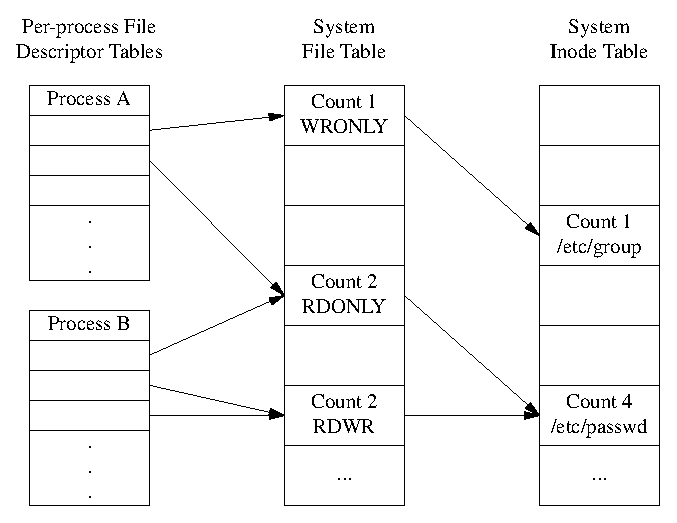
\includegraphics[width=89mm]{img/eps/open_files1.eps}
% This is too big.  I'd have had to shrunk it.
%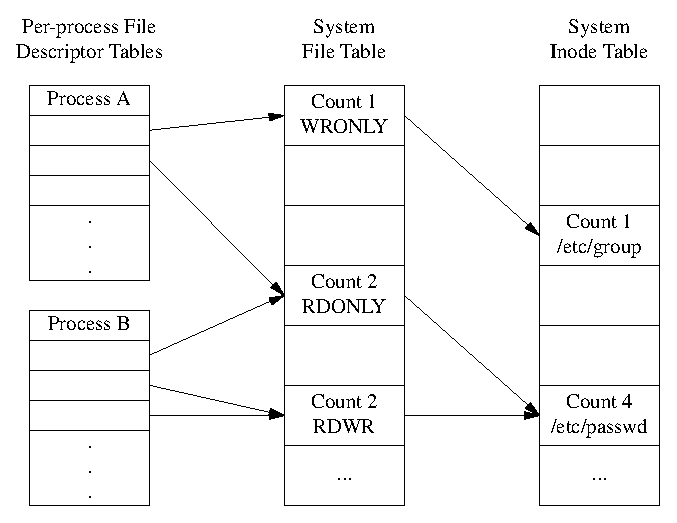
\includegraphics{img/eps/open_files1.eps}
\end{center}
\end{slide}

\hlabel{OPENFILETABLES}

\begin{itemize}
\item This is a simplified view of the kernel tables that deal with files.  It
is modeled after a similar picture in [Bach].  Today it is more complicated but
the main idea stays.
\item Each process on the system has its \emph{file descriptor table}.
\item Slots in that table point to the \emph{system file table}.  There is
only one such a table in kernel.  This table carries the opened file mode and
also the \emsl{current file position.} Each \texttt{open} call will create
a new entry in the table. However, file descriptor duplication or inheritance
will lead to sharing of the slots.
\item From the system file table, it is pointed to the \emph{system inode
table}.  Nowadays the table contains so called \emph{vnodes} -- \emph{virtual
nodes} but that is not relevant for us now. For more info,
see page \pageref{VFS}.
\item The system file table represents an additional level of indirection so
that different processes can share the file position.
\item When opening a file via an \texttt{open} call, a new slot in both the file
descriptor and system file tables is always allocated.  File position sharing in
the same process is achieved via file descriptor duplication where more
descriptors share the same system file table slot.  If a file position sharing
is needed among multiple processes, that is achieved via the \texttt{fork}
call, and it is explained on page \pageref{FDSHARING}.
\item To see how the file descriptor table looks like for given process,
use \texttt{lsof} (Linux distributions, macOS) or \texttt{pfiles} (Solaris)
programs. They will come handy for debugging file descriptor leaks or
inheritance/redirection issues.
\end{itemize}

%%%%%

\pdfbookmark[1]{open}{open}

\begin{slide}
\sltitle{Opening a file: \texttt{open()}}
ifdef([[[NOSPELLCHECK]]], [[[
\texttt{int \funnm{open}(const char *\emph{path}, int \emph{oflag},
... );}
]]])
\begin{itemize}
\item opens a file \texttt{path}, returns its file descriptor. The
\texttt{oflag} is an OR combination of the following flags:
    \begin{itemize}
    \item \texttt{O\_RDONLY}/\texttt{O\_WRONLY}/\texttt{O\_RDWR} \dots{}
    open for reading, writing, or both
    \item \texttt{O\_APPEND} \dots{} append only
    \item \texttt{O\_CREAT} \dots{} create the file if it does not exist
    \item \texttt{O\_EXCL} \dots{} fail if the file exists (for use with
    \texttt{O\_CREATE})
    \item \texttt{O\_TRUNC} \dots{} truncate the file (write permission
    needed)
    \item \dots{}
    \end{itemize}
\item with \texttt{O\_CREAT}, the third parameter \emph{mode}
defines the access mode for the newly create file
\end{itemize}
\end{slide}

\hlabel{OPEN}

\begin{itemize}
\item The first available file descriptor is always used.
\item When \texttt{O\_CREAT} is used, the \emph{mode} is modified using the
current mask that can be changed using the \texttt{umask} system call
(the \texttt{umask} shell command is a wrapper of this system call)
-- those bits in \emph{mode}, that are also set in the process umask,
are nullified.
The default umask value is typically (and historically) \texttt{022}.
We recommend that you always set it to \texttt{077} in your profile script.
Never do that for root though otherwise you may end up with a system in
a non-supported configuration -- installed software may not be possible to run
by non-privileged users, what worked before may stop working, etc.
\item If the \emph{mode} argument is required and not specified, you get
whatever is presently on the stack or in the CPU register used to pass the
argument.  Both flags and mode are stored in the system file table, see page
\pageref{OPENFILETABLES}.
\item Macros for use with \emph{mode} can be usually found in the manual page
for \texttt{chmod(2)}, and you can find them also in the \texttt{sys/stat.h}
header file (or in another file included from it) where the standard requires
them to be.
\item A no longer needed slot in the file descriptor or system file table is
zeroed out before its reuse.
\item There are other flags as well:
\begin{itemize}
\item \texttt{O\_SYNC} (\texttt{O\_DSYNC}, \texttt{O\_RSYNC}) \dots{} the call
returns after the data is physically stored (synchronized I/O).
\texttt{O\_DSYNC} is for writing synchronization only, \texttt{O\_RSYNC} for
reading.
\item \texttt{O\_NOCTTY} \dots{} when opening a terminal by a process without a
controlling terminal, the terminal being opened does not become one.
\item \hlabel{O_NONBLOCK} \texttt{O\_NONBLOCK} \dots{} if reading or writing
cannot be satisfied right away, calls \texttt{read}/\texttt{write} will fail
instead of getting blocked and waiting for the completion.  \texttt{errno} is
set to \texttt{EAGAIN} in such a case.
\end{itemize}
\item One cannot use \texttt{O\_RDONLY | O\_WRONLY} for both reading and writing
as historically, implementations used 0 for the read-only flag.  The standard
defines that only one of those three flags may be used.
\item It is possible to open and create a file for writing so that writing is
disallowed by its mode.  It will work for the initial file opening but any
subsequent attempts to write will fail.
\item You need write permission to use \texttt{O\_TRUNC}.
\item The behavior of \texttt{O\_EXCL} without using \texttt{O\_CREAT} at the
same time is undefined.
\item For file locking, the \texttt{fcntl} call is used, see page
\pageref{FCNTL}.
\end{itemize}

%%%%%

ifdef([[[NOSPELLCHECK]]], [[[
\pdfbookmark[1]{creat}{creat}
]]])

\begin{slide}
\sltitle{Creating a file}
\texttt{int \funnm{creat}(const char *\emph{path}, mode\_t \emph{mode});}
\begin{itemize}
\item the function is equivalent to:\\
\texttt{open(path, O\_WRONLY|O\_CREAT|O\_TRUNC, mode);}
\end{itemize}
\texttt{int \funnm{mknod}(const char *\emph{path}, mode\_t \emph{mode},
dev\_t \emph{dev});}
\begin{itemize}
\item creates a device special file
\end{itemize}
\texttt{int \funnm{mkfifo}(const char *\emph{path}, mode\_t \emph{mode});} 
\begin{itemize}
\item creates a named pipe
\end{itemize}
\end{slide}

\hlabel{MKFIFO}
\hlabel{CREAT}

\begin{itemize}
\item The \texttt{open} call allows opening of a regular file, device, or named
pipe.  However, it (and \texttt{creat} as well) can only create a regular file,
so you need the other two calls for non-regular files.
\item The test of a file's existence using the flag \texttt{O\_EXCL} and its
subsequent creation if it did not exist, is an atomic operation.  You can use
that for lock files but only with the \texttt{open} call, not \texttt{creat},
because \texttt{creat} lacks the flags specification.
\item You need extra privileges to create device special files (e.g. to be a
root).
\end{itemize}

%%%%%

\pdfbookmark[1]{read, write}{readwrite}

\begin{slide}
\sltitle{Reading and writing files: \texttt{read()}, \texttt{write()}}

ifdef([[[NOSPELLCHECK]]], [[[
\texttt{ssize\_t \funnm{read}(int \emph{fd}, void *\emph{buf},
size\_t \emph{nbyte});}
]]])
\begin{itemize}
\item attempts to read \emph{nbyte} bytes of data from the object referenced by
the descriptor \emph{fd} into the buffer pointed to by \emph{buf}
\item returns the number of bytes actually read, 0 on \texttt{EOF}, -1 on error
\end{itemize}

ifdef([[[NOSPELLCHECK]]], [[[
\texttt{ssize\_t \funnm{write}(int \emph{fd}, const void *\emph{buf},
size\_t \emph{nbyte});}
]]])
\begin{itemize}
\item attempts to write \emph{nbyte} of data to the object referenced by the
descriptor \emph{fd} from the buffer pointed to by \emph{buf}
\item number of bytes which were written is returned, -1 on error
\end{itemize}
\end{slide}

\hlabel{READCALL}

\begin{itemize}
\setlength{\itemsep}{0.8\itemsep}
\item For any Unix system, a file is just a sequence of bytes without any inner
structure.
\item The \emsl{behavior of \texttt{read} and \texttt{write} depends on the type of
the file} (regular, device, pipe, or socket) and whether the file is in a
blocking or non-blocking mode (flag \texttt{O\_NONBLOCK} on file opening, see
page \pageref{O_NONBLOCK}).
\item For both calls there are quite a few situations that may happen, and
those most important are listed in the next few paragraphs.  For the full
disclosure, consult the standard or a manual page on your system.
\item \texttt{read} returns a non-zero number of bytes less than \emph{nbyte} if
less than \emph{nbyte} bytes remain in a file, if the call was interrupted
by a signal, or if the file is a pipe, device, or socket and there is less than
\emph{nbyte} bytes available at the moment.  For the last case, if there is no
data, a blocking \texttt{read} will block unless some data gets available, a
non-blocking \texttt{read} returns -1 and sets \texttt{errno} to
\texttt{EAGAIN}.
\item \texttt{write} returns a non-zero number of bytes less than \emph{nbyte}
if less then \emph{nbyte} bytes can fit into the file (e.g. disk full), if the call
was interrupted by a signal, or if \verb#O_NONBLOCK# was set and only part of
the data fits into a pipe, socket, or a device; without \verb#O_NONBLOCK#
the call will block until all the data can be written.  If nothing can be
written, a blocking \texttt{write} blocks until writing data is possible, a
non-blocking call returns -1 and sets \texttt{errno} to \texttt{EAGAIN}.
\item \emsl{Important exceptions for pipes} are listed on page
\pageref{NAMEDPIPE}.
\item
If \texttt{read} or \texttt{write} returns a non-zero number less than
\texttt{nbyte} due to an error, a repeated call returns -1 and sets
\texttt{errno}.
\item If \texttt{read} or \texttt{write} are interrupted before they manage to
read or write, respectively, at least one byte, the call returns -1 and sets
\texttt{errno} to \texttt{EINTR}.  Note that there is a difference if the call
manages to read or write, respectively, at least one byte -- see the paragraphs
above.
\item \texttt{O\_APPEND} guarantees an atomic write to the end of a file on a
local filesystem, i.e. \emsl{every} write will add data to the file end (so
called \emph{append-only} file).
\end{itemize}

%%%%%

\pdfbookmark[1]{close}{close}

\begin{slide}
\sltitle{Closing a file: \texttt{close()}}
\texttt{int \funnm{close}(int \emph{fildes});}
\begin{itemize}
\item releases \texttt{fildes}, if it was the last descriptor for a file
opening, closes the file
\item if the number of links is 0, the file data is released
\item if the last pipe descriptor is closed, any remaining data is lost
\item on process termination, an implicit \texttt{close} is called on all
descriptors
\end{itemize}
\end{slide}

\begin{itemize}
\item Note that the file data is released only after the number of links gets to
0 \emsl{and} if the file was opened before, when closing it.  It means that you
can \texttt{rm} all hard links to a specific file but if a process has the file
still open, the file data remains on the disk until the process closes the file
or terminates.
\item If a process needs a temporary file, it can create it, \texttt{unlink}
(see page \pageref{UNLINK}) it right away, and work with it using the existing
file descriptor.  When the file descriptor is closed (and all of its possible
duplicates), the file data is released.
\item Even \texttt{close} may fail.  For example, some filesystems may write the
data on file closure (NFS), and if that write fails, \texttt{close} fails.
In such case the error code should be used only for diagnostics. There is no
point in retrying because the descriptor might have been allocated for something
else in the meantime.
\item Usually, esp. on local file systems, \texttt{close} returns right away,
however there are situations when \texttt{close} will only return after an
event or certain time, e.g. for TCP sockets with certain options set.
\item If you forget to close file descriptors when you no longer need them,
and it is a long living process, a daemon perhaps, depending on the system
configuration you may hit memory starvation as the system memory will be filled
with an ever growing file descriptor table.
\item \hlabel{SIMPLE_CAT} A very simple \texttt{cat(1)} program:
\example{read/cat.c}
\end{itemize}

%%%%%

\begin{slide}
\sltitle{Example: copy files}
\begin{alltt}
{\footnotesize
#include <fcntl.h>
#include <unistd.h>

int main(int argc, char *argv[])
\{
    char buf[4096];
    int inf, outf;
    ssize\_t ilen;

    inf = \emprg{open}(argv[1], O\_RDONLY);
    outf = \emprg{creat}(argv[2], 0666);
    while ((\emblue{ilen} = \emprg{read}(inf, buf, sizeof (buf))) > 0)
            \emprg{write}(outf, buf, \emblue{ilen});

    \emprg{close}(inf); \emprg{close}(outf);
    return (0);
\}
}
\end{alltt}
\end{slide}

\begin{itemize}
\item The example above is complete.  You can cut-and-paste, compile, and run
it.  Obviously, due to the slide size constraint, it is missing several error
checks otherwise needed for a well behaved utility, like checking \texttt{argc}
before using \texttt{argv}, or checking return values for \texttt{open},
\texttt{creat}, \texttt{read}, and \texttt{write}, and reporting possible
errors.
\item It is not efficient to read and write by a few bytes as each system call
costs a certain overhead, independent on the size of the processed block.  It is
much better to read and write larger blocks, say 8-1024KB.  You can
\texttt{strace(1)} a \texttt{cat} command on Linux to see what blocks they use
for \texttt{read}.  It may be around 128 kilobytes.  The following example,
\example{read/cat.c}, has an option \texttt{-b} for setting the read block size;
you can try different block sizes, including 1, on a reasonable big file (use
\texttt{mkfile(1)} on BSD/macOS or \texttt{fallocate(1)} on Linux to create an
arbitrarily large file), and use \texttt{time(1)} to measure the system call
overhead.
\item If you need to work with little pieces of data read from files, you can
use stream oriented functions that internally buffer the data -- \texttt{fopen},
\texttt{fread}, \dots  However, those functions are prohibited in your semester
assignment and at the exam.
\item Note that we always only write as many bytes as we actually read.  See
page \pageref{READCALL} for more information on when we can read/write less data
than requested.
\end{itemize}

%%%%%
\begin{slide}
\sltitle{Working with a named pipe (FIFO)}

\begin{itemize}
\item it may not be possible to create a FIFO on a distributed filesystem (e.g.
NFS or AFS)
\item you need to know the semantics of opening a FIFO
  \begin{itemize}
  \item opening a FIFO for just reading will block until a writer (aka producer)
  shows up, unless one already exists.
  \item opening a FIFO for just writing will block until a reader (aka consumer)
  shows up, unless one already exists.
  \item this behavior can be adjusted using a flag \texttt{O\_NONBLOCK}
  \end{itemize}
\item semantics for reading and writing is a bit more complicated, see
the notes below this slide.
  \begin{itemize}
  \item same as for a conventional, unnamed, pipe (will be later)
  \end{itemize}
\end{itemize}
\end{slide}

\hlabel{NAMEDPIPE}

\begin{itemize}
\item A named pipe is created using the system call \texttt{mkfifo}, see page
\pageref{MKFIFO}.  Using an unnamed pipe is described later on page
\pageref{PIPE}.
\item A consumer is a process that opens a file/pipe for reading, a producer
opens a file/pipe for writing.
\item It is possible to open a named pipe for reading and writing at the same
time.  The same process thus can write to the pipe and then read the same data
from it.
\item If the pipe is not yet open for writing by any process, to open the pipe
for reading without blocking on the call, one needs to use \texttt{O\_NONBLOCK},
see page \pageref{O_NONBLOCK}.  Without that flag the consumer will block
waiting for a producer (in the \texttt{open} system call, not in
\texttt{read}!).
\item However, trying to read a previously opened pipe that has no producer
results in a return value of 0, indicating the end of file -- the process will
not block waiting for a producer.  It is irrelevant whether the pipe was opened
in a blocking or non-blocking mode.
\item When writing to a pipe without a consumer (i.e. the producer opened the
pipe when there was at least one existing consumer), the kernel will send the
producer a signal \texttt{SIGPIPE} (``broken pipe'').  See the following
example.  For simplicity, we are using an unnamed pipe but a named pipe
would behave in the same manner.  The \texttt{date(1)} command never
reads anything from its standard input so it is guaranteed that the producer,
\texttt{dd(1)}, will be writing to a pipe without a consumer.  If a process is
killed by a signal, the shell provides a signal number added to 128 as its
return value, and \texttt{kill -l} understands that:

\begin{verbatim}
bash$ dd if=/dev/zero | date
Sun Mar  2 01:03:38 CET 2008
bash$ echo ${PIPESTATUS[@]}
141 0
bash$ kill -l 141
PIPE
\end{verbatim}

Another possibility with named pipes:

\begin{verbatim}
$ mkfifo fifo
$ while [ 1 ]; do cat /etc/passwd; done >> /tmp/bigpasswd
^C
$ read < fifo &
[1] 65946
$ cat /tmp/bigpasswd > fifo
[1]+  Done                    read < fifo
$ echo $?
141
\end{verbatim}

\item When opening a pipe for writing only with \texttt{O\_NONBLOCK} and without
an existing consumer, the call returns -1 and \texttt{errno} is set to
\texttt{ENXIO}.  This asymmetry in opening a pipe for reading in non-blocking
mode (see above) is due to the fact that it is not desirable to have data in a
pipe that may not be read in a short period of time.  The Unix system does not
allow for storing pipe data for an arbitrary length of time.  By asymmetry we
mean that the system allows consumers without producers but it tries to avoid
writers without existing readers.  Without the \texttt{O\_NONBLOCK} flag, the
process will block while waiting for a consumer.
\item  If you want to create a process that sits on a named pipe and processes
data from producers, you need to open it with the flag \texttt{O\_RDWR} even
if you do not intend to write to it.  If you do not use the flag, you might end
up with \texttt{read} returning 0 after all producers, perhaps only temporarily,
disappear, which could be solved by busy waiting.  A much better solution would
be to use the \texttt{select} call, see page \pageref{SELECT}.
\item Writing data of length \texttt{PIPE\_BUF} bytes or less
(\texttt{limits.h}) is guaranteed as atomic, i.e. data will not be intermingled
with data written by other writers.  For example, on Linux kernel 6.x it is 4096
bytes, on Solaris 11 it is 5120 bytes, and on FreeBSD 15.0 it is only 512 bytes.
It is obvious from the above that if less or equal than \texttt{PIPE\_BUF}
bytes is written, the data is always written whole or the operation fails,
and if \texttt{O\_NONBLOCK} is set and the whole data buffer cannot be written
(for example, a pipe can hold only a limited number of bytes), the call will fail.
\item A pipe has no file position, data is always appended to a pipe.
\item All the information here applies to a unnamed pipes as well, see page
\pageref{PIPE}.
\end{itemize}

%%%%%

\pdfbookmark[1]{lseek}{lseek}

\begin{slide}
\sltitle{Setting file position: \texttt{lseek()}}
\texttt{off\_t \funnm{lseek}(int \emph{fildes}, off\_t \emph{offset},
int \emph{whence});}
\begin{itemize}
\item will set the file offset for reading and writing in an already
opened file associated with a file descriptor \emph{fildes}
\item based on value of \texttt{whence}, the file offset is set to:
    \begin{itemize}
    \item \texttt{SEEK\_SET} \dots{} the value of \emph{offset}
    \item \texttt{SEEK\_CUR} \dots{} current position plus \emph{offset}
    \item \texttt{SEEK\_END} \dots{} size of the file plus \emph{offset}
    \end{itemize}
\item returns the resulting offset (i.e. from the file beginning)
\item \texttt{lseek(fildes, 0, SEEK\_CUR)} only returns the current file
position
\end{itemize}
\end{slide}

\begin{itemize}
\item \hlabel{LSEEK} The first byte is at position 0.  If it makes sense, you may
use a negative number for setting the \emph{offset}.  Example:
\example{read/lseek.c}.
\item It is legal to move beyond the end of the file.  If data is written there,
the file size will be set accordingly, the ``holes'' will be read as zeros.
Note that just changing the file position will not increase the file size.
\item You can get the file size via \texttt{lseek(fildes, 0, SEEK\_END)}.
\item The most common operations with \texttt{lseek} are three: setting the
position from the beginning of a file, setting the position to the end of a
file, and getting the current file position (0 with \texttt{SEEK\_CUR}).
\item There is no I/O involved when calling \texttt{lseek}.
\item You can obviously use the return value of \texttt{lseek} not only for
subsequent calls to \texttt{read} and \texttt{write} but also for another call
to \texttt{lseek}.
\item \hlabel{BIG_FILE} Beware of files with holes as it may lead to problems
with backing up the data.  Example: \example{read/big-file.c} demonstrates that
moving a sparse file may end up in an actual storage data occupation increase.
It greatly depends on the system you run, what archiving utility is used, and
their versions.  Some utilities provide the means to preserve holes, for example,
\texttt{dd} with \texttt{conv=sparse}, \texttt{tar} with \texttt{-S},
\texttt{rsync} with \texttt{--sparse}, etc.
\item Beware of confusing the parameters.  The second line below looks OK but
the arguments are in reversed order.  What is more, \texttt{SEEK\_SET} is
defined as 0 and \texttt{SEEK\_CUR} is 1, so the file position is not moved
which is not by itself a disastrous thing, which makes it more difficult to find
it:

\begin{verbatim}
lseek(fd, 1, SEEK_SET);
lseek(fd, SEEK_SET, 1);    /* WRONG!!! */
\end{verbatim}
\end{itemize}

%%%%%

\pdfbookmark[1]{truncate}{truncate}

\begin{slide}
\sltitle{Change file size: \texttt{truncate()}}
\texttt{int \funnm{truncate}(const char *\emph{path}, off\_t \emph{length});\\
int \funnm{ftruncate}(int \emph{fildes}, off\_t \emph{length});}
\begin{itemize}
\item causes the regular file to be truncated to a size of precisely
\emph{length} bytes.
\item if the file was larger than \emph{length}, the extra data is lost
\item if the file was previously shorter, it is extended, and the extended part
reads as null bytes
\end{itemize}
\end{slide}

\begin{itemize}
\item Truncating the file when opening  can be achieved via the
\texttt{O\_TRUNC} flag in \texttt{open}, see page \pageref{OPEN}.
\end{itemize}

%%%%%

ifdef([[[NOSPELLCHECK]]], [[[
\pdfbookmark[1]{dup, dup2}{dup}
]]])

\begin{slide}
\sltitle{Descriptor duplication: \texttt{dup()}, \texttt{dup2()}}
\texttt{int \funnm{dup}(int \emph{fildes});}
\begin{itemize}
\item creates a copy of the file descriptor \emph{fildes}, using the
lowest-numbered unused descriptor.  Returns the new descriptor.
\item same as \texttt{fcntl(fildes, F\_DUPFD, 0);} (will be later)
\end{itemize}
\texttt{int \funnm{dup2}(int \emph{fildes}, int \emph{fildes2});}
\begin{itemize}
\item duplicates \texttt{fildes} to \texttt{fildes2}.
\item almost the same as:\\
\texttt{close(fildes2);\\ fcntl(fildes, F\_DUPFD, fildes2);}
\end{itemize}
\end{slide}

\hlabel{DUP_CALL}

\begin{itemize}
\item We already know that the first available file descriptor is used when
opening and creating file, see page \pageref{OPEN}.
\item The original and duplicated file descriptors share the same slot in the
system file table (see page \pageref{OPENFILETABLES}), i.e. they share the file
position and read/write mode.
\item The equivalent for \texttt{dup2} is not fully equivalent.  If
\emph{fildes} is equal to \emph{fildes2}, \texttt{close(fildes2)} does not
happen and \texttt{dup2} returns \texttt{fildes2} right away.
\end{itemize}

%%%%%

\begin{slide}
\sltitle{Example: implement shell redirection}
\begin{itemize}
\item \verb#$ program <in >out 2>> err#
\end{itemize}
\begin{verbatim}
close(0);
open("in", O_RDONLY);
close(1);
open("out", O_WRONLY | O_CREAT | O_TRUNC, 0666);
close(2);
open("err", O_WRONLY | O_CREAT | O_APPEND, 0666);
\end{verbatim}
\begin{itemize}
\item \verb#$ program >out 2>&1#
\end{itemize}
\begin{verbatim}
close(1);
open("out", O_WRONLY | O_CREAT | O_TRUNC, 0666);
close(2);
dup(1);
\end{verbatim}
\end{slide}

\begin{itemize}
\item Note the flag \texttt{O\_APPEND} used to implement the \texttt{>>}
redirection.
\item \hlabel{REDIRECT} Another example of \texttt{dup} use will be provided when
we start working with pipes.  The first redirection example from the slide
(without \texttt{stderr}) is in \example{read/redirect.c}.  In that example, the
\texttt{execl} call replaces the current process image with the
program passed in the first argument.  We got ahead of ourselves here though, we
will learn about the \texttt{exec} calls on page \pageref{EXEC}.
\item To fully understand how redirection works it is good to draw the file
descriptor table for each step and where the slots point to.  In
the \nth{2} example in the slide above, we have the initial state, after
\texttt{close(1)} and \texttt{open("out", ...)}, and the final state, as
follows:

\begin{verbatim}
+-------+              +-------+              +-------+
|   0   +-> stdin      |   0   +-> stdin      |   0   +-> stdin
+-------+              +-------+              +-------+
|   1   +-> stdout ==> |   1   +-> "out"  ==> |   1   +-> "out"
+-------+              +-------+              +-------+    /
|   2   +-> stderr     |   2   +-> stderr     |   2   +---'
+-------+              +-------+              +-------+
\end{verbatim}

\item You need to pay attention to the state of descriptors. The \nth{2} example
above will not work if the descriptor 0 is already closed, as 
\texttt{open} returns 0 (the first available descriptor) and \texttt{dup} fails
while trying to duplicate an already closed descriptor.  Possible
solutions:

\begin{alltt}
close(1);
if ((fd = open("out", O\_WRONLY | O\_CREAT | O\_TRUNC, 0666)) == 0)
        dup(0);
close(2);
dup(1);
if (fd == 0)
        close(0);
\end{alltt}

or

\begin{alltt}
fd = open("out", O\_WRONLY | O\_CREAT | O\_TRUNC, 0666);
if (fd != 1) \{
        dup2(fd, 1);
        close(fd);
\}
dup2(1, 2);
\end{alltt}
\end{itemize}

%%%%%

\pdfbookmark[1]{fcntl, ioctl}{fcntlioctl}

\begin{slide}
\sltitle{Manipulate file descriptors and devices: \texttt{fcntl()},
\texttt{ioctl()}} \texttt{int \funnm{fcntl}(int \emph{fildes}, int
\emph{cmd}, ...);}
\begin{itemize}
\item file descriptor duplication
\item setting descriptor and file status flags
\item advisory and possibly mandatory locking
\end{itemize}

\texttt{int \funnm{ioctl}(int \emph{fildes}, int \emph{request}, ... );}
\begin{itemize}
\item manipulates the underlying device parameters of special files
\item used as a universal interface for manipulating devices
\item each device defines a set of requests it understands
\end{itemize}
\end{slide}

\hlabel{FCNTL}

\begin{itemize}
\item Example: close standard error output on program execution (exec call):\\
\texttt{fcntl(2, F\_SETFD, FD\_CLOEXEC);}
\item We will see later that descriptors are used for sockets as well, so it is
possible to use \texttt{fcntl} on them, for example to set a non-blocking
socket.  See page \pageref{CONNECT} for more information.
\item Values for \emph{cmd} in \texttt{fcntl}:
\begin{itemize}
\item \texttt{F\_DUPFD} \dots{} duplicate descriptors
\item \texttt{F\_GETFD} \dots{} get file descriptor flags.  \texttt{FD\_CLOEXEC}
is the only descriptor flag defined in SUSv4.
\item \texttt{F\_SETFD} \dots{} set file descriptor flags
\item \texttt{F\_GETFL} \dots{} get file opening flags (read/write, append,
\dots)
\item \texttt{F\_SETFL} \dots{} set file opening flags
(\texttt{O\_APPEND}, \texttt{O\_DSYNC}, \texttt{O\_NONBLOCK},
\texttt{O\_R\-SYNC}, and \texttt{O\_SYNC}).
Setting ifdef([[[NOSPELLCHECK]]], [[[RO/RW]]]) is not allowed, and neither are
flags for creation, truncation, and exclusive access.
\item \texttt{F\_GETLK}, \texttt{F\_SETLK}, \texttt{F\_SETLKW} \dots{}
for file locking
\end{itemize}
\item Note the difference between \texttt{fcntl} commands ending with
\texttt{FD} and \texttt{FL}. While the former deal with a file descriptor, the
latter deal with a file opening, i.e. particular slot in the system file table
of opened files. See also the picture on page \pageref{OPENFILETABLES}.
\item Devices may support reading and writing using \texttt{read} and
\texttt{write}, and mapping files to memory (\texttt{mmap}, see page
\pageref{MMAP}), all other operations on devices (e.g. setting parameters,
locking, or eject) are performed using the \texttt{ioctl} system call.
\item When setting flags, always get the present flags first.  Even when you
know the flags are zero, you never know how the code will be modified in the
future, and what other flags are possibly added.  So, you should always use
something like the following when setting a new flag:

\begin{verbatim}
flags = fcntl(fd, F_GETFL);
fcntl(fd, F_SETFL, flags | O_APPEND);
\end{verbatim}

or better with proper error checks:

\begin{verbatim}
if (((flags = fcntl(fd, F_GETFL)) == -1) ||
    (fcntl(fd, F_SETFL, flags | O_APPEND) == -1)) {
        err(...);
}
\end{verbatim}

\dots similarly when removing a flag.
\end{itemize}

%%%%%

\pdfbookmark[1]{stat, fstat}{stat}

\begin{slide}
\sltitle{Get file status information: \texttt{stat()}}
\setlength{\baselineskip}{0.9\baselineskip}
ifdef([[[NOSPELLCHECK]]], [[[
\texttt{int \funnm{stat}(const char *\emph{path}, struct stat *\emph{buf});\\
int \funnm{fstat}(int \emph{fildes}, struct stat *\emph{buf});}
]]])
\begin{itemize}
\item for a file specified by a path or a file descriptor, returns a structure
containing file information, such as:
\begin{itemize}
\item \texttt{st\_ino} \dots{} i-node number
\item \texttt{st\_dev} \dots{} ID of device containing file
\item \texttt{st\_uid}, \texttt{st\_gid} \dots{} user/group ID of owner
\item \texttt{st\_mode} \dots{} file type and mode
\item \texttt{st\_size}, \texttt{st\_blksize}, \texttt{st\_blocks}
\dots{} total size in bytes, preferred block size for filesystem I/O,
and number of 512 byte blocks allocated
\item \texttt{st\_atime}, \texttt{st\_mtime}, \texttt{st\_ctime}
\dots{} time of last access, last modification, and last i-node modification
\item \texttt{st\_nlink} \dots{} number of hard links
\end{itemize}
\end{itemize}
\end{slide}

\begin{itemize}
\item You may be able to instruct the system not to update the file access time
when reading from a file, with granularity per file system.  This option is
useful on file systems where there are large numbers of files and performance is
more critical than updating the file access time (which is rarely ever
important).  It may also come in handy if your filesystem is on a medium with a
limited number of erase/write cycles -- a CompactFlash, for example.  If your
system supports it, it will be the \texttt{noatime} option for the \texttt{mount}
command.  See the manual page. Some systems (Linux based) support a non-portable
\texttt{open} syscall flag to set this per file opening, based on some
conditions.
\item \emph{Metadata} is information about the file -- access mode, access
times, length, owner, group, etc.  Metadata does \emsl{not} include the file
data itself, or the file name as the file data can be accessed through
several different hard links and those hardlinks are in the data of directories.
In other words, metadata is data about the actual file data.
\item Metadata can be read even when the process has no rights to read the file
data.
\item These functions do not provide file descriptor flags or flags from the
system file table. These functions are about file information as stored on some
mountable media.
\item \texttt{st\_ctime} is not the creation time but the change time -- the
last modification of the inode.
\item The UNIX norm does not specify the ordering of the \texttt{struct stat}
members, nor does it prohibit adding new ones.
\item \hlabel{STAT} Example: \example{stat/stat.c}
\item You can call \texttt{fstat} on file descriptors 0, 1, and 2 as well.  Unless
redirected before, you will get information on the underlying terminal device
(e.g. \texttt{/dev/ttys011} on macOS).  Example: \example{stat/stat012.c}.
\end{itemize}


%%%%%

\pdfbookmark[1]{lstat}{lstat}

\begin{slide}
\sltitle{Get file status information (2)}
\begin{itemize}
\item for a file type, in \texttt{<sys/stat.h>} there are
constants \verb#S_IFMT# (bit mask for the file type bit field), \verb#S_IFBLK#
(block device), \verb#S_IFCHR# (character device), \verb#S_IFIFO#
(FIFO), \verb#S_IFREG# (regular), \verb#S_IFDIR# (directory), and
\verb#S_IFLNK# (symlink). 
\item macros for file type checking: \verb#S_ISBLK(m)#,
\verb#S_ISCHR(m)#, \verb#S_ISFIFO(m)#, \verb#S_ISREG(m)#,
\verb#S_ISDIR(m)#, and \verb#S_ISLNK(m)#. 
\item access right masks: \verb#S_IRUSR# (owner has read permission),
\verb#S_IWGRP# (group has write permission), etc.
\end{itemize}
ifdef([[[NOSPELLCHECK]]], [[[
\texttt{int \funnm{lstat}(const char *\emph{path}, struct stat
*\emph{buf});}
]]])
\begin{itemize}
\item if \emph{path} is a symlink, \texttt{stat()} returns information about the
file the symlink refers to. \texttt{lstat()} function returns information about the link
itself.
\end{itemize}
\end{slide}

\begin{itemize}
\item The file type and access mode are stored together in the
\verb#st_mode# member and that is why the aforementioned macros exist.
\item \texttt{S\_IFMT} specifies those bits that store the file type, and the
macros are not bit masks but values.  So, the test for the specific file type is
needed to be done like the following (extra parentheses are needed due to the
operator precedence): \texttt{((st\_mode~\&~S\_IFMT)~==~S\_IFREG)}.  All macros
are defined in the spec and thus portable.
\item Example: \example{stat/filetype.c}
\end{itemize}

%%%%%

ifdef([[[NOSPELLCHECK]]], [[[
\pdfbookmark[1]{utime, futimens, utimensat}{utime}
]]])

\begin{slide}
\sltitle{Setting file times}
ifdef([[[NOSPELLCHECK]]], [[[
\texttt{int \funnm{utime}(const char *\emph{path},
const struct utimbuf *\emph{times});}
]]])
\begin{itemize}
\item changes file last access (\texttt{atime}) and modification
(\texttt{mtime}) times
\item cannot change i-node status change time (\texttt{ctime})
\item calling process must have write permission for the file
\end{itemize}
ifdef([[[NOSPELLCHECK]]], [[[
\texttt{int \funnm{futimens}(int fd, const struct timespec times[2]);}
\texttt{int \funnm{utimensat}(int fd, const char *path, \\
const struct timespec times[2], int flag);}
]]])
\begin{itemize}
\item allow to set both access and modification time
\end{itemize}
\end{slide}

\begin{itemize}
\item The \texttt{utime} call is mostly used the by \texttt{cp} and \texttt{mv}
commands and also archive utilities to make sure the times are the same for the
originals and copies. (e.g. \texttt{tar} or \texttt{rsync}).
\item The \texttt{futimens} and \texttt{utimensat} offer greater deal of
flexibility. They allow to set the time to current time, using special
constant in the \texttt{timespec} structure. Also, \texttt{utimensat()}
has a flag that controls whether to work directly on a symlink or its target.
Lastly, they offer greater precision (nanoseconds), compared to legacy
interfaces such as \texttt{utime()} (seconds) or \texttt{utimes()}
(microseconds).
\item The \texttt{touch} command offers access to the above interfaces.
\item There is an excellent section \emph{1.7 Dates and Times} in [Rochkind]
that goes through various representations of time in Unix systems, and functions
that use those.  It is 12 pages of good stuff, highly recommended if you ever
need to work with time in C and/or Unix.
\end{itemize}

%%%%%

ifdef([[[NOSPELLCHECK]]], [[[
\pdfbookmark[1]{link, unlink, rename}{link}
]]])

\begin{slide}
\sltitle{File name manipulations}
\texttt{int \funnm{link}(const char *\emph{path1}, const char *\emph{path2});}
\begin{itemize}
\item creates a new link (aka hard link), i.e. a directory entry, named
\emph{path2} to file \emph{path1}.  Hard links cannot span filesystems (use
\funnm{symlink} for that).
\end{itemize}
\hlabel{UNLINK} \texttt{ int \funnm{unlink}(const char *\emph{path});}
\begin{itemize}
\item deletes a name (i.e. a directory entry) and after deleting the last link to
the file and after closing the file by all processes, deletes the file data.
\end{itemize}
\texttt{int \funnm{rename}(const char *\emph{old}, const char *\emph{new});}
\begin{itemize}
\item changes the file name (i.e. one specific link) from \emph{old} to
\emph{new}.  Works within the same filesystem only.
\end{itemize}
\end{slide}

\begin{itemize}
\item It is better said again -- \emsl{Unix does not have a delete call for
files}.  Details are on page \pageref{FILEDELETE}.
\item The call \texttt{link} creates hardlinks, i.e. a relation between a file
name and an i-node number.  I-node numbers are unique within a filesystem so for
links between filesystems, symlinks are needed.  A number of hardlinks to a
specific file is only limited by the size of the \texttt{st\_nlink} member of
\texttt{struct stat}, and the specification does not specify the size, it only
says its type \texttt{nlink\_t} is an integer value.
\item The parameter \emph{path2} must not exist.  So, you cannot rename using
the \texttt{link} call.
\item \texttt{unlink} does not work on directories, see \texttt{rmdir} on
p\pageref{RMDIR}.
\item The shell command \texttt{mv} uses \texttt{rename} to move objects within
the same filesystem.  To move files between filesystems, a file needs to be
copied first, then \texttt{unlink}ed from the originating filesystem (the whole
operation is not atomic).
\item \texttt{rename} renames symlinks, not the files those symlinks point to.
\item There is also a more generic call \texttt{remove}, see page
\pageref{REMOVE}.
\end{itemize}

%%%%%

ifdef([[[NOSPELLCHECK]]], [[[
\pdfbookmark[1]{symlink, readlink}{symlink}
]]])

\begin{slide}
\sltitle{Symbolic links}
\texttt{int \funnm{symlink}(const char *\emph{path1},
const char *\emph{path2});}
\begin{itemize}
\item make a new symbolic name from \emph{path2} $\rightarrow$ \emph{path1}.
\item \emph{path1} may span filesystems, and may not exist at all
\end{itemize}
ifdef([[[NOSPELLCHECK]]], [[[
\texttt{int \funnm{readlink}(const char *\emph{path}, char *\emph{buf},
size\_t \emph{bufsz});}
]]])
\begin{itemize}
\item put maximum of \emph{\texttt{bufsz}} bytes from the symlink target path
to \texttt{\emph{buf}}
\item returns the number of bytes written to \texttt{\emph{buf}}.
\item The path written to \texttt{\emph{buf}} is \emsl{not} terminated
by \verb#'\0'#
\end{itemize}
\end{slide}

\begin{itemize}
\item The shell command \texttt{ln} uses either the \texttt{symlink} or
\texttt{link} syscall depending on whether the \texttt{-s} option was used.
\item Calling \texttt{unlink} on a hardlink will not release the file data if
other hardlinks exist. You can delete the symlink's target in which case you
end up with a \emph{broken link}.
\item \texttt{readlink} is useful in the situation where you want to
\texttt{unlink} the symlink's target.
\item On some systems (e.g. macOS) there is a \texttt{readlink} command that
will display symlink target:
\begin{verbatim}
$ ls -l /etc/aliases
lrwxr-xr-x  1 root  wheel  15 Oct 24  2017 /etc/aliases -> postfix/aliases
$ readlink /etc/aliases
postfix/aliases
\end{verbatim}
\item \emph{\texttt{bufsz}} is typically set as 1 byte less than the buffer
size to accommodate the terminating \texttt{NULL} character.
\item See \example{readlink/readlink.c} and fix the problem therein.
\item There is also \texttt{readlinkat()} that operates on a file descriptor.
\end{itemize}

%%%%%

ifdef([[[NOSPELLCHECK]]], [[[
\pdfbookmark[1]{mkdir, rmdir, opendir, readdir, closedir}{dirfncs}
]]])

\hlabel{RMDIR}

\begin{slide}
\sltitle{Working with directories}
\texttt{int \funnm{mkdir}(const char *\emph{path}, mode\_t \emph{mode});}
\begin{itemize}
\item attempts to create an empty directory \emph{path} with entries
'\texttt{.}' and '\texttt{..}'
\end{itemize}
\texttt{int \funnm{rmdir}(const char *\emph{path});}
\begin{itemize}
\item deletes directory \emph{path}.  The directory \emsl{must} be empty.
\end{itemize}
ifdef([[[NOSPELLCHECK]]], [[[
\texttt{DIR *\funnm{opendir}(const char *\emph{dirname});}\\
\texttt{struct dirent *\funnm{readdir}(DIR *\emph{dirp});}\\
\texttt{int \funnm{closedir}(DIR *\emph{dirp});}
]]])
\begin{itemize}
\item sequentially reads directory entries
\item structure \texttt{dirent} contains:
    \begin{itemize}
    \item \texttt{d\_ino} \dots{} i-node number
    \item \texttt{d\_name} \dots{} file name
    \end{itemize}
\end{itemize}
\end{slide}

\begin{itemize}
\item Directory items are not ordered and
\texttt{readdir} is allowed to return them in arbitrary order depending on the
filesystem implementation.  \texttt{NULL} is returned on failure
and \texttt{errno} is set.  \texttt{NULL} is also returned upon reaching the end
of a directory but in that case, \texttt{errno} is not changed.
\item \texttt{readdir} is a stateful function.  To read the directory from the
beginning again, \texttt{rewinddir} can be used.  If you want to read the
directory from multiple threads, use the reentrant version, \texttt{readdir\_r}.
\item Some (very) old systems might support reading a directory via a normal
\texttt{read} call.  In that case, of course, you need to know the internal
representation of the directory data so the use of this is questionable.  Linux
does not allow this at all.
\item \texttt{d\_ino} might not be very useful if the directory is a
mountpoint; this member contains the i-node number of the directory where the
filesystem is mounted and not the root of the mounted filesystem as one might
expect.
\item \hlabel{D_TYPE} Some system have a \texttt{struct dirent} member
\texttt{d\_type}.  It can have values of \texttt{DT\_REG}, \texttt{DT\_DIR},
\texttt{DT\_FIFO} etc., see the man page for \texttt{dirent}.  It was a BSD
specific thing and subsequently copied by other systems, including Linux.
However, it is not part of SUSv4 and thus not portable, unfortunately.
The portable way is to call \texttt{stat} on each directory entry.
\item \texttt{rmdir} does not work on directories that are not empty.  You have
to remove all entries before you can delete a directory.  It might be tempting
to use something like \texttt{system("rm -r xxx")}, e.g. invoke a shell to
run the \texttt{rm} command etc., however this should be avoided as it is prone
to errors (the environment and the directory name might be hard to sanitize)
and might have security implications.
\item \hlabel{REMOVE} The specification also defines \texttt{remove} which
behaves like \texttt{unlink} for files and as \texttt{rmdir} for directories.
\end{itemize}

%%%%%

\begin{slide}
\sltitle{Example: read a directory}
\begin{alltt}
int
main(int argc, char *argv[])
\{
    DIR *d;
    struct dirent *de;

    for (int i = 1; i < argc; i++) \{
        if ((d = \emprg{opendir}(argv[i])) == NULL) \{
                warn("%s", argv[i]); continue;
        \}
        while ((de = \emprg{readdir}(d)) != NULL)
            printf("%s\bs{}n", de->d_name);
        \emprg{closedir}(d);
    \}
\}
\end{alltt}
\end{slide}

\begin{itemize}
\item The \texttt{ls} command is based on a similar loop.  It is missing code to
tell whether NULL means an error or an end of a directory.
\item Example (with the correct use of \texttt{errno}):
\example{readdir/readdir.c}
\end{itemize}

%%%%%

ifdef([[[NOSPELLCHECK]]], [[[
\pdfbookmark[1]{chdir, fchdir, getcwd}{pwd}
]]])

\begin{slide}
\sltitle{Change working directory}
\begin{itemize}
\item every process has its current working directory.  When a process refers to
a file using a relative path, the reference is interpreted relative to the
current working directory of the process.
\item the working directory is inherited from the process parent
\end{itemize}
\texttt{int \funnm{chdir}(const char *\emph{path});}\\
\texttt{int \funnm{fchdir}(int \emph{fildes});}
\begin{itemize}
\item changes the working directory for the process
\end{itemize}
\texttt{char *\funnm{getcwd}(char *\emph{buf}, size\_t \emph{size});}
\begin{itemize}
\item stores the absolute path to the current working directory to \emph{buf},
its \emph{size} must be at least one byte longer than the path length.
\end{itemize}
\end{slide}

\begin{itemize}
\item The current working directory for a process is stored in a process
structure in kernel, usually it is a link to the directory's \emph{vnode}.
For more info about vnodes see page \pageref{VFS}.
\item The descriptor for \texttt{fchdir} is from \texttt{open} called on the
directory (i.e. not from \texttt{opendir}).
\item There is also a function \texttt{chroot} which changes the root
directory of a calling process to a new one.  It is often used in various server
implementations to limit access to the specific subtree.  For example, for an
FTP server.  You have to be careful though and make sure it is not possible to
escape from the chrooted subtree and access other parts of the filesystem.  The
function is also not a part of SUSv4.
\begin{itemize}
\item Other, more generic ways of isolation are provided in available systems,
and differ from each other greatly.  For example, there are jails in Free\-BSD,
zones in Solaris, sandboxing in macOS, LXC in Linux (that is what Docker is
based on there), etc.
\end{itemize}
\end{itemize}

%%%%%

\pdfbookmark[1]{access}{access}

\begin{slide}
\sltitle{Check permissions for access: \texttt{access()}}
ifdef([[[NOSPELLCHECK]]], [[[
\texttt{int \funnm{access}(const char *\emph{path}, int \emph{amode});}
]]])
\begin{itemize}
\item checks whether the calling process can access the file \emph{path}
\item \emph{\texttt{amode}} is an OR-combination of constants
    \begin{itemize}
    \item \verb#R_OK# \dots{} read permission test
    \item \verb#W_OK# \dots{} write permission test
    \item \verb#X_OK# \dots{} execution permission test
    \item \verb#F_OK# \dots{} file existence test
    \end{itemize}
\item in contrast to \texttt{stat()}, the result depends on the process's
\texttt{RUID} and \texttt{RGID}
\item \emsl{never use this call, it cannot be used in a safe way.  See the notes
below.}
\end{itemize}
\end{slide}

\begin{itemize}
\item This call applies mechanism of access right testing to a specific file for
the calling process.
\item The function was meant for an SUID process to verify whether the user
running the process would have had access to a file if it was not for the SUID
privileges.  However, there is an inherent security hole in this approach.
The test and the subsequent action on the file is not an atomic operation.
This is called the time-of-check to time-of-use (TOCTOU) problem,
see \url{https://en.wikipedia.org/wiki/Time-of-check\_to\_time-of-use}.
An attacker could possibly \texttt{unlink} the file and immediately symlink it
to a different file to what it actually had no rights to manipulate with.
If the timing is right, the SUID process will operate on that other file.
\\
The correct solution is not to use the \texttt{access} call but return to the
real UID/GID and try the operation.  For example, if we succeed in opening the
file under the real UID/GID and continue working with the file descriptor, the
file manipulation mentioned above would not gain the attacker anything.
\end{itemize}

%%%%%

ifdef([[[NOSPELLCHECK]]], [[[
\pdfbookmark[1]{chmod, chown}{chmodchown}
]]])

\begin{slide}
\sltitle{Setting file permissions}
ifdef([[[NOSPELLCHECK]]], [[[
\texttt{int \funnm{chmod}(const char *\emph{path}, mode\_t \emph{mode});}
]]])
\begin{itemize}
\item changes permissions of file \emph{path} to \emph{mode}.
\item can be used by the file owner or root
\end{itemize}
ifdef([[[NOSPELLCHECK]]], [[[
\texttt{int \funnm{chown}(const char *\emph{path}, uid\_t \emph{owner},
gid\_t \emph{group});}
]]])
\begin{itemize}
\item changes file owner and group for \emph{path}.  Value of
\texttt{-1} means do not change that ID.
\item only root can change owners so that users could not work around quotas
to disown their files
\item a regular user can change a group of files he/she owns, and must belong to
the target group
\end{itemize}
\end{slide}

\begin{itemize}
\item The \emph{mode} parameter does not contain the file type, of course.  See
\texttt{sys/stat.h} or the \texttt{chmod(2)} manual page for available bit
masks.
\item Only the owner of a file can change its mode.  Mode like
\texttt{rw-rw-rw-} has nothing to do with that.
\item In some implementations, it was possible to pass the file ownership to
someone else.  Today this is usually not allowed.  Just think about how you
could work around a per-user filesystem quota with this.
\end{itemize}

\endinput
